\lhead{\begin{tikzpicture}[remember picture, overlay]
    \node [anchor=100,inner sep=0] (imagenIZQUIERDA) at (current page header area.north)
    {
\includegraphics[width=18cm]{img/Encabezado.PNG}};
    \end{tikzpicture}}
    \rhead{Ángeles-Hurtado}
    \rfoot{\begin{tikzpicture}[remember picture, overlay]
    \node [anchor=140,inner sep=0] (imagenDERECHA) at (current page footer area.south){
\includegraphics[width=18cm]{img/Foot.PNG}};
    \end{tikzpicture}}
    %----------------------------------------------------------------------------------------
    \lfoot{ \thepage}
    % \renewcommand{\labelenumi}{\alph{enumi}.)} 
    %----------------------------------------------------------------------------------------
    %----------------------------------------------------------------------------------------
    %	TITLE SECTION
    %----------------------------------------------------------------------------------------
    
    \setlength{\droptitle}{-5\baselineskip} % Move the title up
    \title{\textbf{Estudio de tiempos y movimientos en el ensamble de un circuito electrónico utilizando diferentes métodos para su optimización }} % Article title
    
     \author{ 
     \textsc{flores martinez ricardo missael}\\ 
    %  Afiliación:
     \texttt{ Instituto Tecnológico de Queretaro } \\ 
     \texttt{ Tecnológico Nacional de México } \\ 
     \texttt{Queretaro, México}\\ 
     \texttt{l22140280@queretaro.tecnm.com} 
     \and 
     \textsc{Ángeles-Hurtado, Luis Alberto}\\ 
    %  Afiliación:
     \texttt{ Instituto Tecnológico de Querétaro } \\ 
     \texttt{ Tecnológico Nacional de México } \\ 
     \texttt{Querétaro, México}\\ 
     \texttt{alb3rt0.ah@gmail.com} 
    }
    
    
    %----------------------------------------------------------------------------------------
    
    % \begin{document}
    
    % Print the title
    \maketitle
    \thispagestyle{fancy}
    
    %----------------------------------------------------------------------------------------
    %	ARTICLE CONTENTS
    %----------------------------------------------------------------------------------------
    
    % \section*{Resumen}
    % \textit{Palabras clave:}
    % El resumen (ancho de página) deberá contener entre 100 y 200 palabras tipo Adobe Devangari 11 puntos.
    
    \begin{abstract}
    \noindent 
    El resumen (ancho de página) deberá contener entre 100 y 200 palabras tipo Adobe Devangari 11 puntos.
    
    \end{abstract}
    % 
    % 
    \textbf{\textit{Palabras clave}}: {First keyword should be the corresponding to the research area according with the authors guide. Maximum of 6 keywords.}
    % \keywords{First keyword should be the corresponding to the research area according with the authors guide. Maximum of 6 keywords.}
    
    \section{Introducción}
    
    % Define estudio de tiempos y movimientos
    % define que es ensamble
    % define que es circuito electronico
    % define el metodo de tiempos predeterminados
    % define optimización
    \begin{itemize}
        \item Estudio de tiempos y movimientos: Es el análisis de métodos, materiales, herramientas e instalación utilizada o que se a de utilizar en la ejecución de un trabajo. 
        \item Ensamble: ensamble implica la colocación de dos o más piezas individuales para la conformación de un producto final. 
        \item Circuito eléctrico: Un circuito eléctrico, por lo tanto, es la interconexión de dos o más componentes que contiene una trayectoria cerrada.
        \item sistema de tiempos predeterminados: conjunto de reglas o métodos para determinar con anticipación la secuencia de sucesos.
        \item Optimización: se refiere a la capacidad de hacer o resolver alguna cosa de la manera más eficiente posible y, en el mejor de los casos, utilizando la menor cantidad de recursos.
    \end{itemize}
    % 
    % 
    \section{Justificación}
    
    \begin{itemize}
        \item el estudio de tiempos y movimientos en el ensamble de un circuito electrónico radica en la búsqueda continua de eficiencia, calidad y competitividad en la industria. Los circuitos electrónicos son componentes fundamentales en una amplia gama de dispositivos y sistemas, desde teléfonos móviles hasta equipos médicos y automóviles. Por lo tanto, optimizar el proceso de ensamble es crucial para garantizar la calidad del producto final, reducir costos y tiempos de producción, y mantener la competitividad en el mercado.
        \item Debe de tener Referencias científicas, URL, tesis, etc.
    \end{itemize}
    % 
    % 
    \section{Descripción del problema}
    \begin{itemize}
        \item En una línea de ensamble de circuitos electrónicos, se ha identificado un aumento en los tiempos de ciclo. Esto se atribuye a una serie de factores, incluyendo la complejidad del proceso de ensamble, la falta de estandarización de métodos de trabajo y la presencia de movimientos innecesarios o ineficientes por parte de los operadores.
    
    Los principales problemas identificados son:
    
    Variabilidad en los tiempos de ciclo: Se observa una alta variabilidad en los tiempos requeridos para ensamblar cada unidad de producto, lo que afecta la capacidad de planificación y programación de la producción.
    Ineficiencias en los movimientos de los operadores: Los operadores realizan movimientos innecesarios, como desplazamientos repetitivos para recoger herramientas o materiales, lo que incrementa los tiempos de ciclo y la fatiga del personal.
        \item Al implementar métodos de optimización, se espera mejorar significativamente la eficiencia y productividad en la línea de ensamble de circuitos electrónicos, reduciendo los tiempos de ciclo y aumentando la calidad del producto final
        \item Debe de tener Referencias científicas, URL, tesis, etc.
    \end{itemize}
    
    \textbf{*La incógnita científica es el elemento cuya solución incrementa el conocimiento científico.}
    % 
    % 
    \section{Fundamentación teórica}
    
    La fundamentación teórica del estudio de tiempos y movimientos en el ensamble de un circuito electrónico se basa en varios principios y teorías relacionados con la gestión de operaciones, la ingeniería industrial y la mejora continua.
    
    \begin{itemize}
        \item Teoría de la medición del trabajo: Esta teoría se centra en métodos y técnicas para medir y analizar el tiempo y el esfuerzo requerido para realizar una tarea específica. El estudio de tiempos predeterminados (MTM), el análisis de movimientos y otros enfoques de medición del trabajo son herramientas fundamentales para identificar áreas de mejora en el ensamble de circuitos electrónicos.
        \item Teoría de la eficiencia del trabajo: Esta teoría se refiere a cómo diseñar y organizar el trabajo de manera que se maximice la productividad y se minimice el desperdicio de recursos. Al aplicar métodos de optimización de tiempos y movimientos, como la eliminación de movimientos innecesarios y la estandarización de métodos de trabajo, se puede mejorar la eficiencia del ensamble de circuitos electrónicos.
        \item Referencias solo de artículos y libros científicos.
    \end{itemize}
    % 
    % 
    \section{Hipótesis}
    
    Hipótesis: La aplicación de diferentes métodos de estudio de tiempos y movimientos en el ensamble de un circuito electrónico conducirá a una mejora significativa en la eficiencia y la productividad de la línea de ensamble.
    
    Fundamento cientifico:
    \begin{itemize}
        \item Principio de mejora continua: La mejora continua es un concepto fundamental en la gestión de operaciones y la ingeniería industrial. Se basa en la premisa de que los procesos pueden ser constantemente mejorados mediante la identificación y eliminación de desperdicios y la optimización de los métodos de trabajo. Al aplicar diferentes métodos de estudio de tiempos y movimientos, como el análisis de movimientos y el diseño de estaciones de trabajo ergonómicas, se pueden identificar áreas de ineficiencia y oportunidades de mejora que conducirán a una mayor eficiencia y productividad en la línea de ensamble de circuitos electrónicos.
        \item Teoría de la medición del trabajo: La medición del trabajo proporciona un marco científico para cuantificar el tiempo y el esfuerzo requeridos para realizar una tarea específica. Métodos como el estudio de tiempos predeterminados (MTM) permiten establecer estándares de tiempo para cada tarea de ensamble, lo que facilita la planificación y programación de la producción. Al aplicar métodos de medición del trabajo de manera sistemática, se pueden identificar y eliminar actividades que agregan poco valor al proceso de ensamble, lo que conduce a una mejora en la eficiencia y la productividad.
        \item Teoría de la ergonomía: La ergonomía se centra en el diseño de lugares de trabajo y tareas para que se adapten a las capacidades y limitaciones humanas. Al diseñar estaciones de trabajo ergonómicas y optimizar la disposición de herramientas y materiales, se puede reducir la fatiga y el estrés de los operadores, lo que contribuye a una mayor eficiencia y productividad en el ensamble de circuitos electrónicos.
    \end{itemize}
    % 
    % 
    \section{Objetivo}
    
    El objetivo general del estudio de tiempos y movimientos en el ensamble de un circuito electrónico es mejorar la eficiencia y la productividad de la línea de ensamble mediante la aplicación de diferentes métodos de optimización.
    
    \subsection{Objetivos específicos }
    
    \begin{itemize}
        \item Identificar y analizar los diferentes pasos y actividades involucrados en el ensamble de un circuito electrónico.
        \item Medir y registrar los tiempos requeridos para cada tarea de ensamble utilizando métodos como el estudio de tiempos predeterminados (MTM).
        \item Analizar los movimientos realizados por los operadores durante el ensamble para identificar oportunidades de optimización y reducción de movimientos innecesarios.
        \item Diseñar y establecer estaciones de trabajo ergonómicas que mejoren la eficiencia y reduzcan la fatiga de los operadores.
        \item Desarrollar un método de trabajo estandarizado y optimizado que describa paso a paso las actividades de ensamble, minimizando la variabilidad en los tiempos de ciclo.
        \item Implementar mejoras basadas en los resultados del estudio de tiempos y movimientos, incluyendo la eliminación de pasos redundantes, la optimización de la disposición de herramientas y materiales, y la estandarización de métodos de trabajo.
        \item Evaluar el impacto de las mejoras implementadas en la eficiencia y la productividad de la línea de ensamble, mediante la comparación de los tiempos de ciclo antes y después de la optimización.
        \item Proporcionar recomendaciones para la mejora continua del proceso de ensamble de circuitos electrónicos, basadas en los hallazgos y resultados del estudio de tiempos y movimientos.
    \end{itemize}
    
    % 
    % 
    \section{Cuerpo (Metodología, modelo matemático, etc.)}
    
    Cada estrategia metodológica se establece acorde a cada objetivo, y por tanto deberá ser desglosada precisada y ordenada claramente. En consecuencia cada objetivo que se presentó en forma de verbo en infinitivo deberá determinar una estrategia en forma de adverbio. Ej. Desarrollar…Desarrollo. Son las actividades ordenadas que tienen como finalidad la prueba de la hipótesis. 
    
    \begin{itemize}
        \item Se debe establecer que se habrá de hacer, como, conque, y donde para obtener la información que permita probar la hipótesis.  
        \item Se debe desglosar de acuerdo a los objetivos específicos. 
        \item Se debe establecer una estrategia metodológica por cada objetivo específico. De manera simplista se podría decir que se cambia el verbo en infinitivo por su respectivo adverbio.
        \item En cada objetivo se debe describir que método, que materiales y que equipo se usará para conseguirlo.
        \item Se deben tener referencias.
    \end{itemize}
    % 
    % 
    \subsection{Prepara tu documento}
    
    Antes de que comiences a utilizar esta plantilla, es recomendable que prepare la información que contendrá en un archivo aparte. 
    Ten preparadas tus gráficas, así como también las tablas aparte, para que sea más fácil integrarlo. 
    Se recomienda fuertemente el uso de \textbf{formato Enhanced Metafile (.emf) para imágenes y gráficas} de resolución óptima. 
    Finalmente, completa y organiza el contenido antes de darle el formato de esta plantilla. 
    
    \subsection{Acrónimos y Abreviaciones}
    
    Los acrónimos y abreviaciones deberán ser definidos únicamente la primera vez que aparecen en el texto, esto para que el lector entienda lo que significan.
    
    \subsection{Ecuaciones}
    
    Las ecuaciones son una excepción a las especificaciones prescritas de esta plantilla. 
    Deberá determinar si su ecuación debe escribirse o no utilizando la fuente Adobe Devangari. 
    Para crear ecuaciones multinivel, puede ser necesario tratar la ecuación como un gráfico e insertarla en el texto después de aplicar el estilo de la platilla.
    Las ecuaciones serán enumeradas de manera consecutiva, y el número de ecuación, entre paréntesis, se colocan al ras de la derecha, utilizando una tabulación derecha. 
    
    \begin{equation}
        \label{eq1}
        x + y = z 
    \end{equation}
    
    Es importante asegurarse de que los símbolos de la ecuación sean definidos antes o inmediatamente después de la ecuación. Utilice “(1)”, en vez de “Eq. 1” al enumerar las ecuaciones, excepto al principio de una oración: “La ecuación (\ref{eq1}) es…”
    
    \section{Resultados y discusión}
    \begin{frame}{Insertando imágenes}
        \begin{figure}
            \centering
            \includegraphics[width=5cm]{11/img/fotoAnalista1.jpeg}
            \caption{resultado}
            \label{fig:enter-label}
             \centering
            \includegraphics[width=5cm]{11/img/fotoAnalista2.jpeg}
            \caption{resultado}
            \label{fig:enter-label}
             \centering
            \includegraphics[width=5cm]{11/img/fotoAnalista3.jpeg}
            \caption{resultado}
            \label{fig:enter-label}
             \centering
            \includegraphics[width=5cm]{11/img/fotoAnalista4.jpeg}
            \caption{resultado}
            \label{fig:enter-label}
        \end{figure}
    \end{frame}
    Antes de comenzar a preparar tu artículo, es importante que lea primero la guía del autor, la cual incluye los temas o apartados que son necesarios para tener tu trabajo completo.
    Una vez completada la edición del texto, el documento está listo para el uso de esta plantilla. En este archivo recién creado, resalte todo el contenido e importe el archivo de texto preparado. Ahora esta listo para estilizar su documento.
    En esta sección se deben presentar todo lo obtenido de la sección 2, incluidas deducciones o efectos del desarrollo. También se podrán incluir subsecciones numeradas de la siguiente forma:
    
    \subsection{Autores y Afiliaciones}
    
    Para distinguir las afiliaciones de los autores, utilice superíndices iniciando con el número 1, 2, etc., sucesivamente, esto dependerá de la cantidad de los departamentos a los que estén afiliados los autores. En caso de que todos los autores pertenezcan a una mismo departamento e institución, utilizar sólo el superíndice 1. 
    
    \subsection{Identificar los encabezados}
    
    Se les recuerda a los autores que los encabezados deben de estar conforme los solicita la guía del autor. De ahí se puede adaptar el trabajo para que sea más fácil de entender para el lector.
    Los encabezados organizan los temas sobre una base relacional y jerárquica. Por ejemplo, el título del documento es encabezado del texto principal porque todo el material posterior se relaciona y elabora sobre este tema. 
    
    \subsection{Tablas y Figuras}
    
    \begin{enumerate}
        \item Posición de las tablas y figuras: Coloque las figuras y las tablas en la parte superior e inferior de las columnas. Evite colocarlos en medio. Las figuras y las tablas grandes pueden abarcar ambas columnas. Los títulos de las figuras deben de estar debajo de las mismas; los títulos de las tablas deben aparecer encima de ellas. Insértese las figuras y los cuadros después de citarse en el texto. Utilice la abreviatura “Fig. 1”, incluso al principio de una oración. 
    \end{enumerate}
    
    \section{Conclusiones}
    
    Se describe aquí el alcance del trabajo, logros obtenidos y perspectivas para el futuro de este. Se sugiere colocar información cuantitativa obtenida.
    
    \section{Agradecimientos}
    
    Es importante darles su debido reconocimiento a los laboratorios, instituciones, organizaciones, entre otros que han sido participes para la culminación de este trabajo. También es importante mencionar, fondos, proyectos, becas, entre otros que se le han otorgado al o los autores para realizar el trabajo de investigación. Ejemplo: “Los autores agradecen al Concejo Nacional de Ciencia y Tecnología por los recursos otorgados…”
    
    \section*{Referencias}
    
    % Para esta platilla, se solicita al autor enumerar las citas de manera consecutiva entre corchetes \cite{YLi2013}. 
    % La puntuación de la oración que sigues sería \cite{Mesaelides2011}. 
    % Refiérase simplemente al número de referencia, como en \cite{Morales2012}, no utilice “Ref. [3]” o “referencia [3]” excepto al principio de una oración: “La referencia [3] fue la primera…”
    Enumere las notas al pie por separado en superíndices. Coloque la nota de pie de en la parte inferior de la columna en la que se citó. No coloque notas al pie en la lista de referencias. Utilice letras para las notas al pie de la tabla.
    A menos de que haya tres autores o más; no utilice “et al.”. Los trabajos que no hayan sido publicados, incluso si han sido presentados para su publicación, deben ser citados como “inéditos”. Los trabajos que han sido aceptados para su publicación deben de citarse como “en prensa”. Poner en mayúscula sólo la primera palabra de un título, excepto los nombres propios y los símbolos de elemento. 
    
    % Otros ejemplos \cite{LAAngeles2021}, \cite{LAAngelesConni}. 
    
    % Ejemplo
    %  @Article{article,
    % 	author = "Author1 LastName1 and Author2 LastName2 and Author3 LastName3",
    % 	title = "Article Title",
    % 	volume = "30",
    % 	number = "30",
    % 	pages = "10127-10134",
    % 	year = "2013",
    % 	doi = "10.3389/fnins.2013.12345",
    % 	URL = "http://www.frontiersin.org/Journal/10.3389/fnins.2013.12345/abstract",
    % 	journal = "Frontiers in Neuroscience"
    % }
    
    % @book{book,
    %   author    = {Author Name}, 
    %   title     = {The title of the work},
    %   publisher = {The name of the publisher},
    %   address   = {The city},
    %   year      = 1993,
    % }
    
    % @incollection{chapter,
    %   author       = {Bauthor Surname}, 
    %   title        = {The title of the work},
    %   editor       = {Editor Name},
    %   booktitle    = {The title of the book},
    %   publisher    = {The name of the publisher},
    %   address      = {The city},
    %   year         = 2002,
    %   pages        = {201-213},
    % }
    
    % @InProceedings{conference,
    %   author = {Cauthor Name and Dauthor Surname and Fauthor LastName},
    %   title = {The title of the work},
    %   booktitle = {The title of the conference proceedings},
    %   year = 1996,
    %   publisher = {The name of the publisher},
    %   editor = {Editor Name1 and Editor Name2},
    %   pages = {41-50},
    % }
    
    % @book{cho,
    %   author       = {Gauthor Name1}, 
    %   title        = {The title of the work},
    %   publisher = {Country code and patent number},
    %   address      = {Patent Country},
    %   year = 2013
    % }
    
    % @book{patent,
    %   author    = {Hauthor Surname1}, 
    %   title     = {The title of the work},
    %   publisher = {Patent number},
    %   address   = {Patent country},
    %   year      = 2010,
    % }
    
    % % please use misc for datasets
    % @misc{dataset, 
    % 	author = "Author1 LastName1 and Author2 LastName2 and Author3 LastName3",
    % 	title = "Data Title",
    % 	year = "2011",
    % 	doi = "10.000/55555",
    % 	URL = "http://www.frontiersin.org/",
    % }
    
     
    \bibliographystyle{ieeetr}
    \bibliography{11/referencias}
    % 
    % 
    %%%%%%%%%%%%%%%%%%%%%%%%%%%%%%%%%%
    \appendix
    %%%%%%%%%%%%%%%%%%%%%%%%%%%%%%%%%%
    % 
    % 
    %%%%%%%%%%%%%%%%%%%%%%%%%%%%%%%%%%%%%%%%
    \centering{\section[\appendixautorefname{}]{Apéndice}}\label{anexo:pines}
    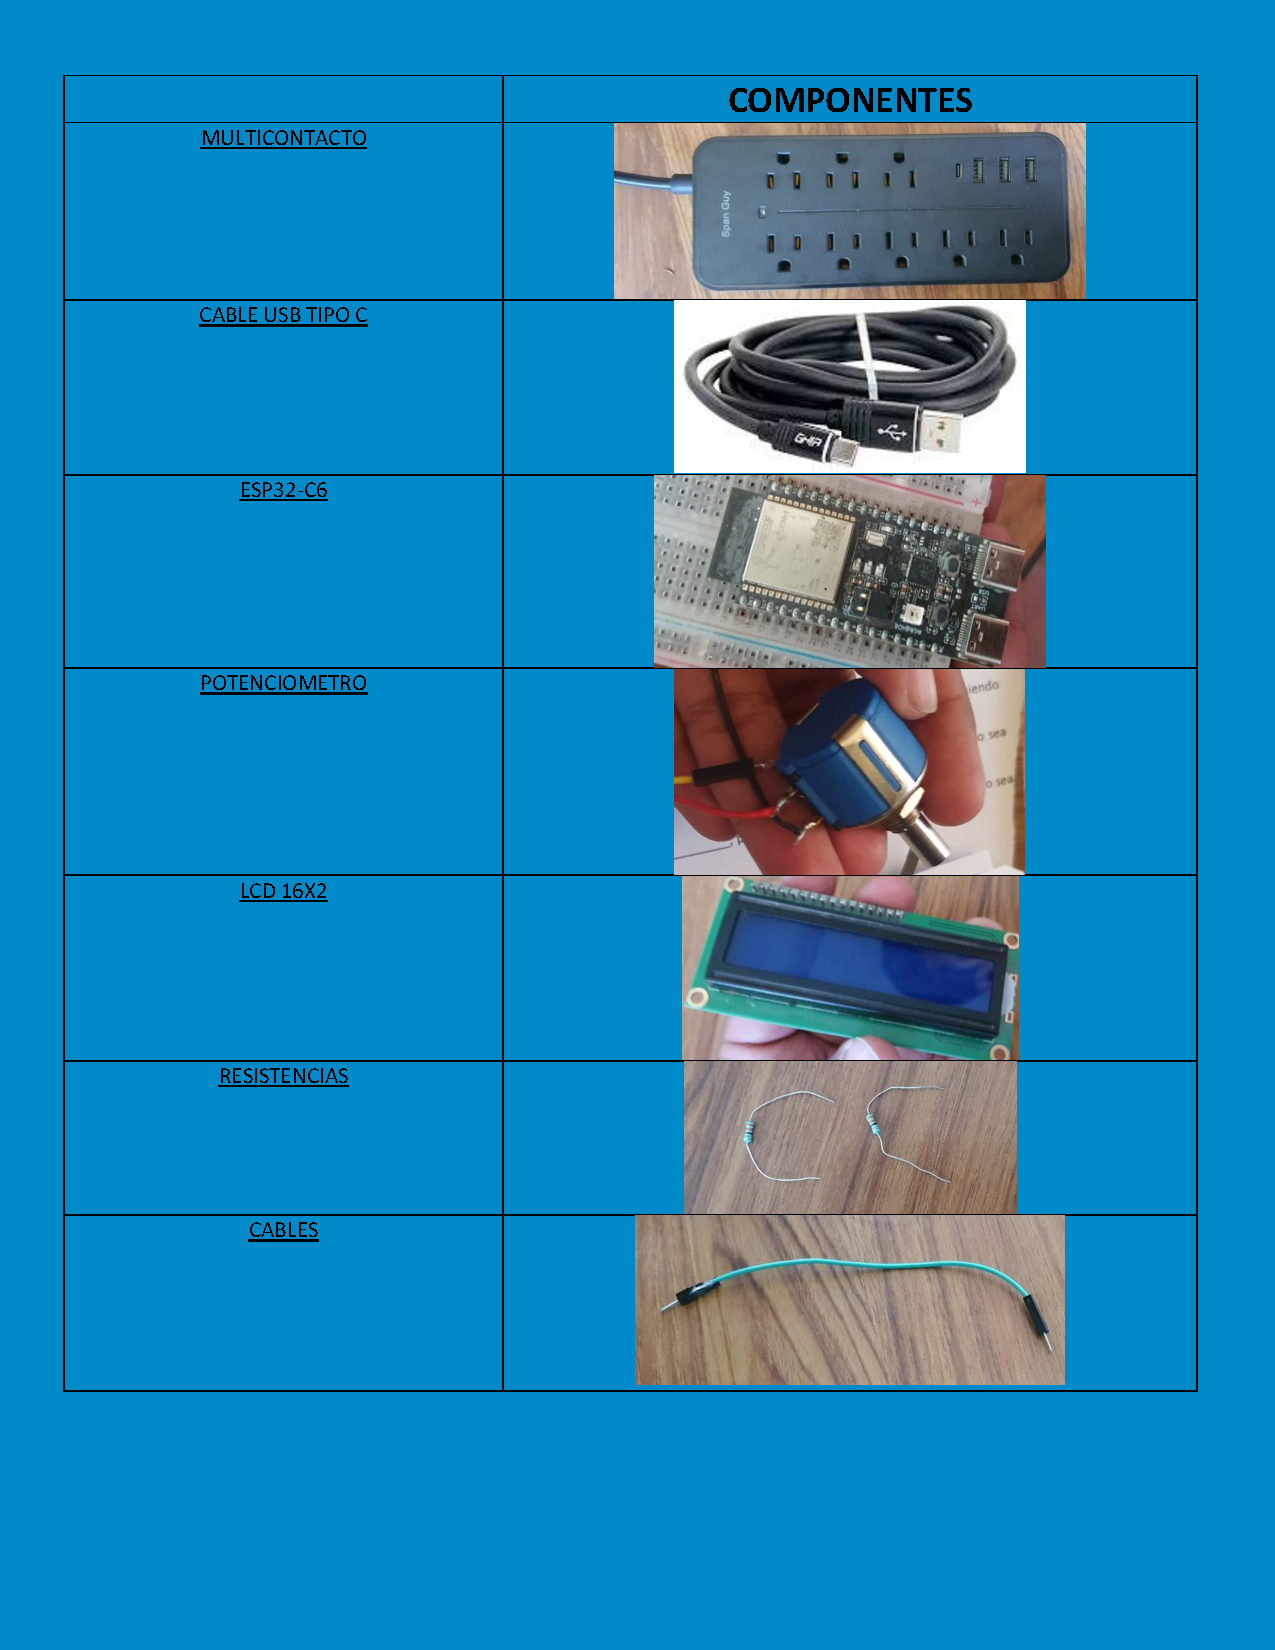
\includepdf[pages=-]{11/img/componentesCircuito.pdf}\label{anexo:componentesCircuito}
    %%%%%%%%%%%%%%%%%%%%%%%%%%%%%%%%%%%%%%%%
    \centering{\section[\appendixautorefname{}]{APÉNDICE}}
    \includepdf[pages=-]{11/img/ensambleCircuitoEsp.pdf}\label{anexo:guiaEnsamble}
    %%%%%%%%%%%%%%%%%%%%%%%%%%%%%%%%%%%%%%%%